\section{Thư viện SFML}
Trong đồ án này, thư viện SFML được sử dụng để thiết kế giao diện người dùng.

\subsection{Giới thiệu về thư viện SFML}
SFML (Simple and Fast Multimedia Library) là một thư viện đa phương tiện được đóng góp từ nhiều người ở cộng đồng, được viết chủ yếu bằng ngôn ngữ C++.

\begin{figure}[H]
\centering{
\includegraphics[scale=0.1]{images/SFMLLogo}}
\caption{Logo của thư viện SFML}
\end{figure}

Thư viện SFML có vài điểm tương đồng với thư viện SDL2 (Simple DirectMedia Layer 2), nhưng được viết chủ yếu theo phương pháp hướng đối tượng nên việc tiếp cận cho các phần mềm hướng đối tượng sẽ dễ dàng hơn nhiều so với SDL2.

Sử dụng thư viện SFML giúp ta viết được các chương trình có thể chạy trên nhiều nền tảng.

\subsection{Các modules của thư viện SFML}
Hiện tại, thư viện SFML cung cấp cho người dùng $5$ modules:
\begin{itemize}
\item \textbf{Audio:} cung cấp các lớp giúp xử lý về âm thanh như: phát một tập tin nhạc hoặc tập tin ghi âm...
\item \textbf{Graphics:} cung cấp các lớp giúp xử lý đồ họa như vẽ hình...
\item \textbf{Network:} cung cấp các lớp giúp xử lý các giao thức mạng nhưu HTTP, FTP...
\item \textbf{System:} cung cấp các lớp giúp xử lý các vấn đề hệ thống như thời gian, Unicode...
\item \textbf{Window:} cung cấp các lớp giúp xử lý cửa sổ sự kiện.
\begin{figure}[H]
\centering{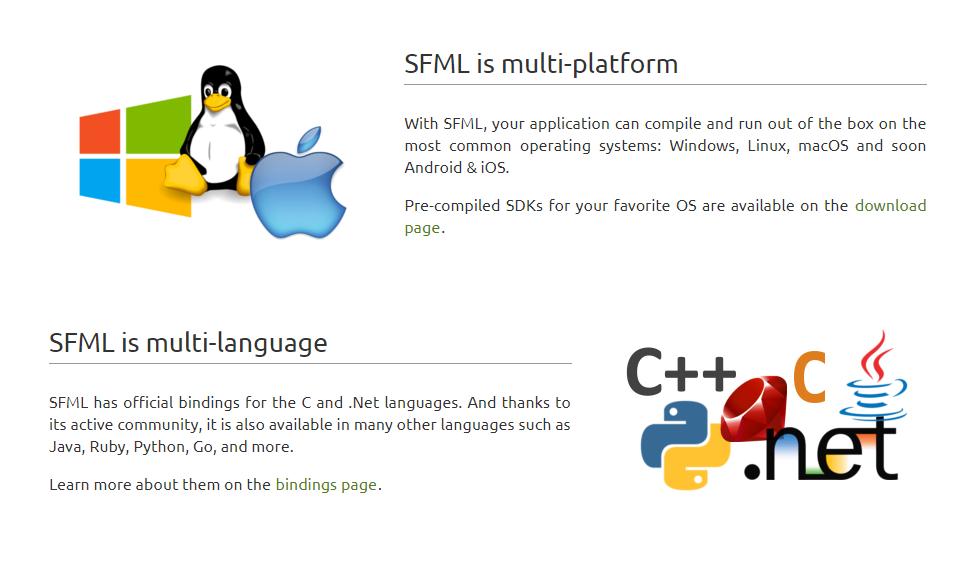
\includegraphics[scale=0.7]{images/sfmldetails}}
\caption{Chi tiết thư viện SFML. Nguồn: \url{gamedevspot.net}}
\end{figure}
\end{itemize}
